\documentclass{article}
\usepackage{fontspec}

% Used to embed Sage code in latex
%\usepackage{sagetex}


% Math Environment
\usepackage{euler}        % Euler font
\usepackage{amsmath}      % Math macros
\usepackage{amssymb}      % Math symbols
\usepackage{unicode-math} % Unicode support

% Physics Environment
\usepackage{physics}


\usepackage[makeroom]{cancel} % Used to cancel terms in algebraic equations
\usepackage{ulem} % Different underline environments
\usepackage{polynom} %Polynomial long division

% Typesetting Rules
\setlength\parindent{0em}
\setlength\parskip{0.618em}
\usepackage[a4paper,lmargin=1in,rmargin=1in,tmargin=1in,bmargin=1in]{geometry}
\setmainfont[Mapping=tex-text]{Helvetica Neue LT Std 45 Light}

% Common Macros
\newcommand\N{\mathbb{N}}
\newcommand\Z{\mathbb{Z}}
\newcommand\Q{\mathbb{Q}}
\newcommand\R{\mathbb{R}}
\newcommand\C{\mathbb{C}}
\newcommand\A{\mathbb{A}}
\def\res{\mathop{\text{Res}}\limits}

% Color
\usepackage[dvipsnames]{xcolor}
\usepackage{pagecolor}
% \definecolor{DeepMossGreen}{HTML}{394820}
% \pagecolor{DeepMossGreen}
% \color{Goldenrod}

\usepackage{graphicx}

\begin{document}

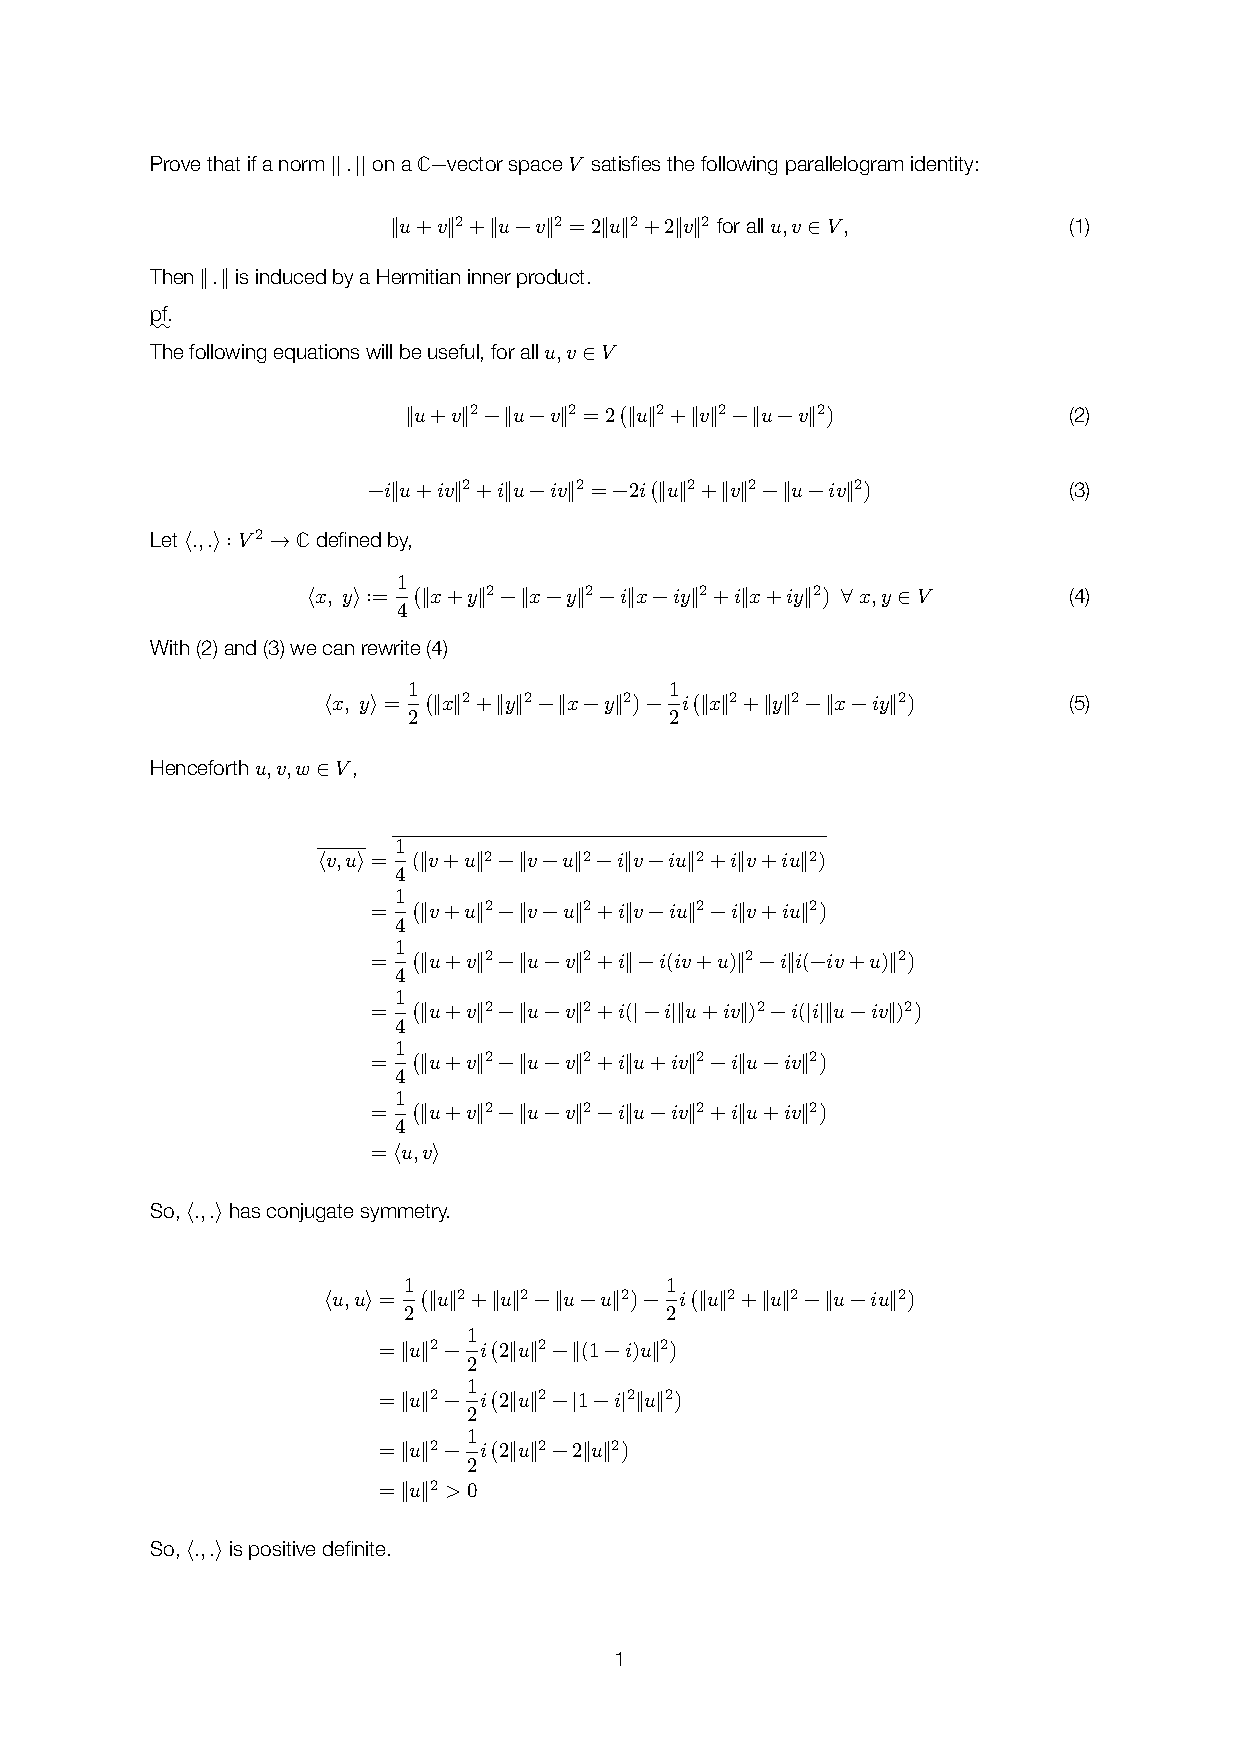
\includegraphics[width=\textwidth]{q1.png}

\uwave{pf.}

Let $\{\vb{e}_i\}_{i=1}^n$ is be standard basis of $\R^n$.

Let $f: E\subset \R^n\rightarrow \R$, such that
\[\exists M_i \in \R: \forall \vb{x} \in E,  |(D_i f)(\vb{x})|\leq
  M_i\quad  (1\leq i\leq n).\]

Let $M = \max \{M_i\}_{i=1}^n$, let $\varepsilon >0$, let $\vb{h} = \sum_{i= 1}^n h_i \vb{e}_i :
\bigg|\sum_{i=1}^n h_i\bigg| < \frac{\varepsilon}{M}$.

Let $\vb{v_0} = 0$, and $v_k = \sum_{i=1}^k h_i\vb{e}_i\quad (1\leq k
\leq n)$, then
\begin{equation}f(\vb{x}+\vb{h})-f(\vb{x}) = \sum_{i=1}^n
  f(\vb{x}+\vb{v_{i}}) - f(\vb{x}+\vb{v_{i-1}})\end{equation}
Since $\vb{v_i} = \vb{v_{i-1}}+h_i\vb{e}_i$, the Mean Value Theorem
(5.10) shows that
\[f(\vb{x}+\vb{v_{i}}) - f(\vb{x}+\vb{v_{i-1}}) = h_i(D_i f)(\vb{x}+
  \vb{v_{i-1}} + \theta_i h_i \vb{e}_i) \]

for some $\theta_i\in (0,1)$. Then we can write,
\[|f(\vb{x}+\vb{h})-f(\vb{x})| = |\sum_{i=1}^n
  h_i(D_i f)(\vb{x}+
  \vb{v_{i-1}} + \theta_i h_i \vb{e}_i)| \leq \sum_{i=1}^n
  |h_i|M_i < M\bigg|\sum_{i=1}^n h_i\bigg| < \varepsilon\]

So $f$ is continuous on $E\quad \blacksquare$
\end{document}




%%% Local Variables:
%%% mode: latex
%%% TeX-master: t
%%% End:
